\subsection{Tokenization}

\cite{BanglaGPT:2}A meaningful unit of text is a token. Words are mostly considered as tokens in NLP. According to the token, a process of breaking a text is known as the process of tokenization.
indicnlp.tokenize: This is a module in the IndicNLP library with the function to deal text in more Indian languages including Bengali.

\textbf{indic\_tokenize.trivial\_tokenize}: It carries out the text in the following trivial tokenize: divides text into meaningful individual words or punctuation symbols.

The first step in BPE training is identifying the distinct set of words included in the corpus, after which the vocabulary is compiled using all the symbols used to represent those words Below is an illustration of the tokenize function.

\begin{figure}[H]
    \centering
    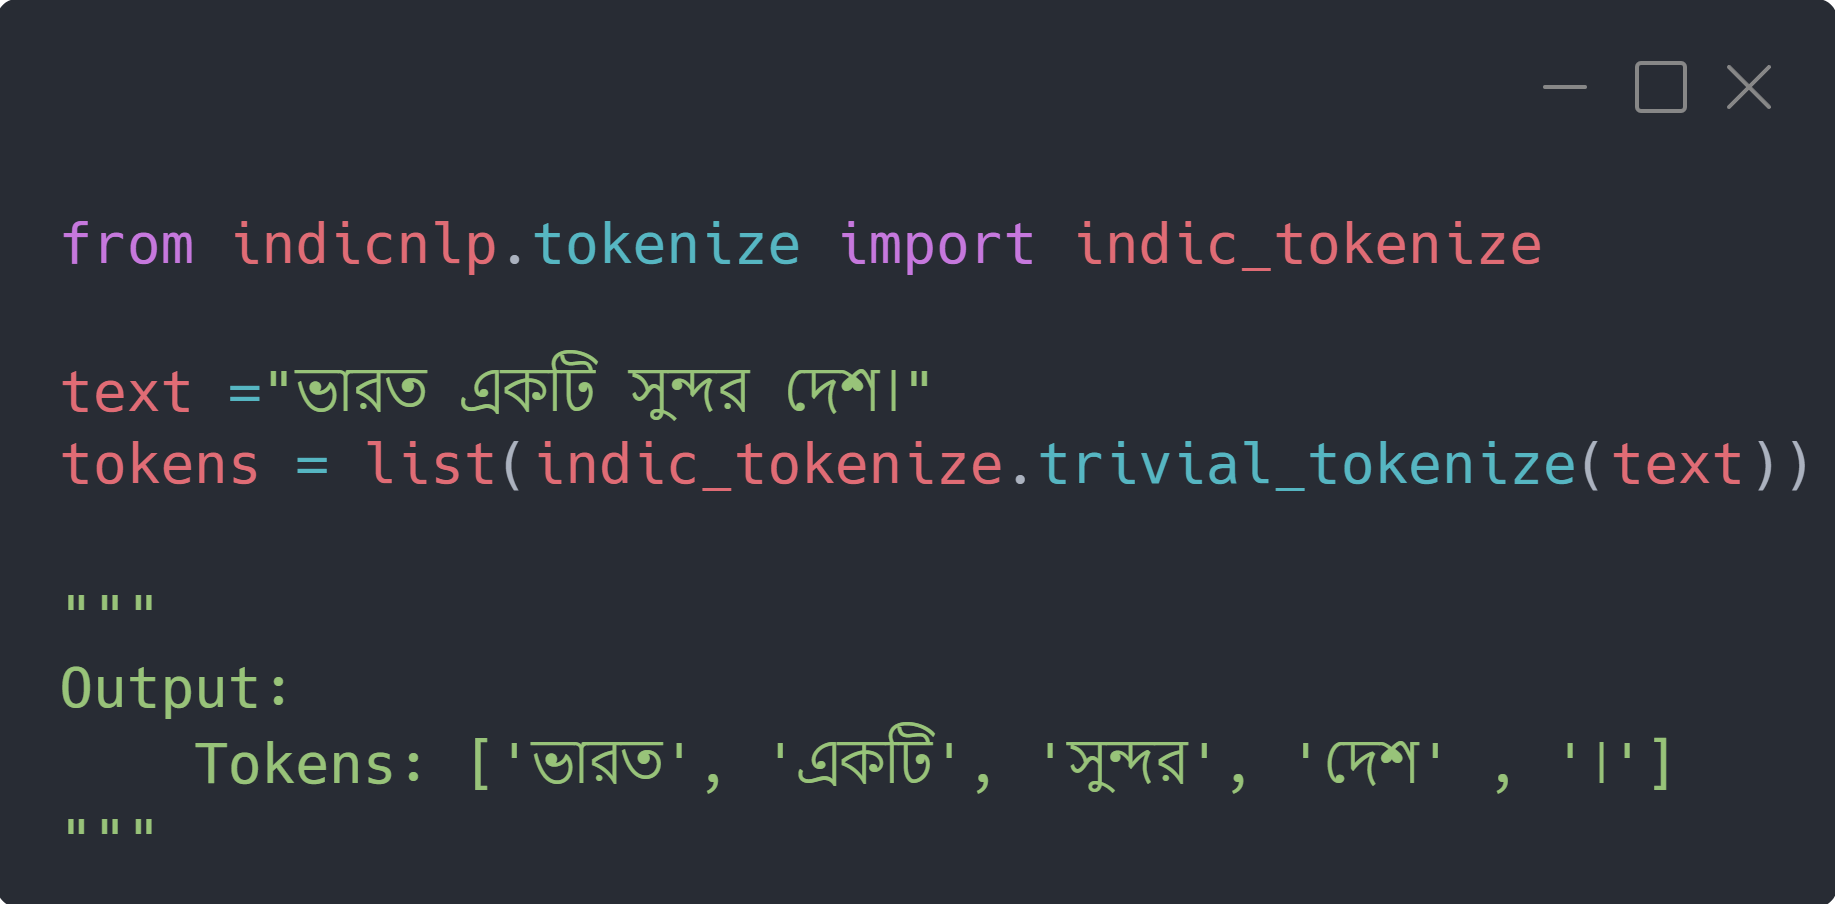
\includegraphics[width=0.8\linewidth]{Attachments/Figures/tokenizer_figure1.png}
    \caption{Illustration of the tokenization process for Bengali text.}
\end{figure}